\section{Strategy}

A camera model is a projection model which describes a mathematical relationship between points in 3D space and its projection onto an image plane. In order to accurately model a camera, we must first understand the general construction of a camera. 




The Tsai camera model builds upon the pinhole camera model, which is one of the simplest and most commonly used camera models.

\subsection{Camera Model}

The 

A pinhole camera is a simple camera without a lens. Instead, it relies on the use of a tiny hole as the aperture of the camera, and light rays pass through the hole, projecting an inverted image onto the 

\begin{figure}[h!]
    \centering
    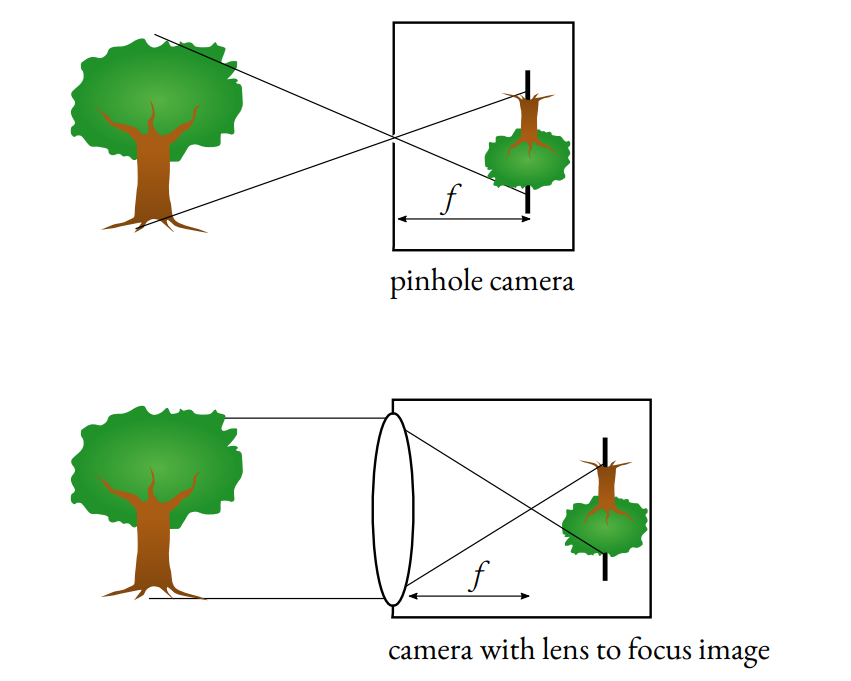
\includegraphics[width=0.7\textwidth]{images/pinhole_vs_lens}
    \caption{Difference between a pinhole camera and a lens camera.}
\end{figure}



There are a few assumptions which are made by the pinhole camera model:
\begin{itemize}
    \item T
\end{itemize}

The pinhole camera model does not accurately describe the true workings of a camera, as some of the  effects that the model fails to account for can be compensated the errors which results from these assumptions are sufficiently small to be neglected if a high quality camera is used. Additionally,

\subsection{Nomenclature}

\begin{figure}[h!]
    \centering
    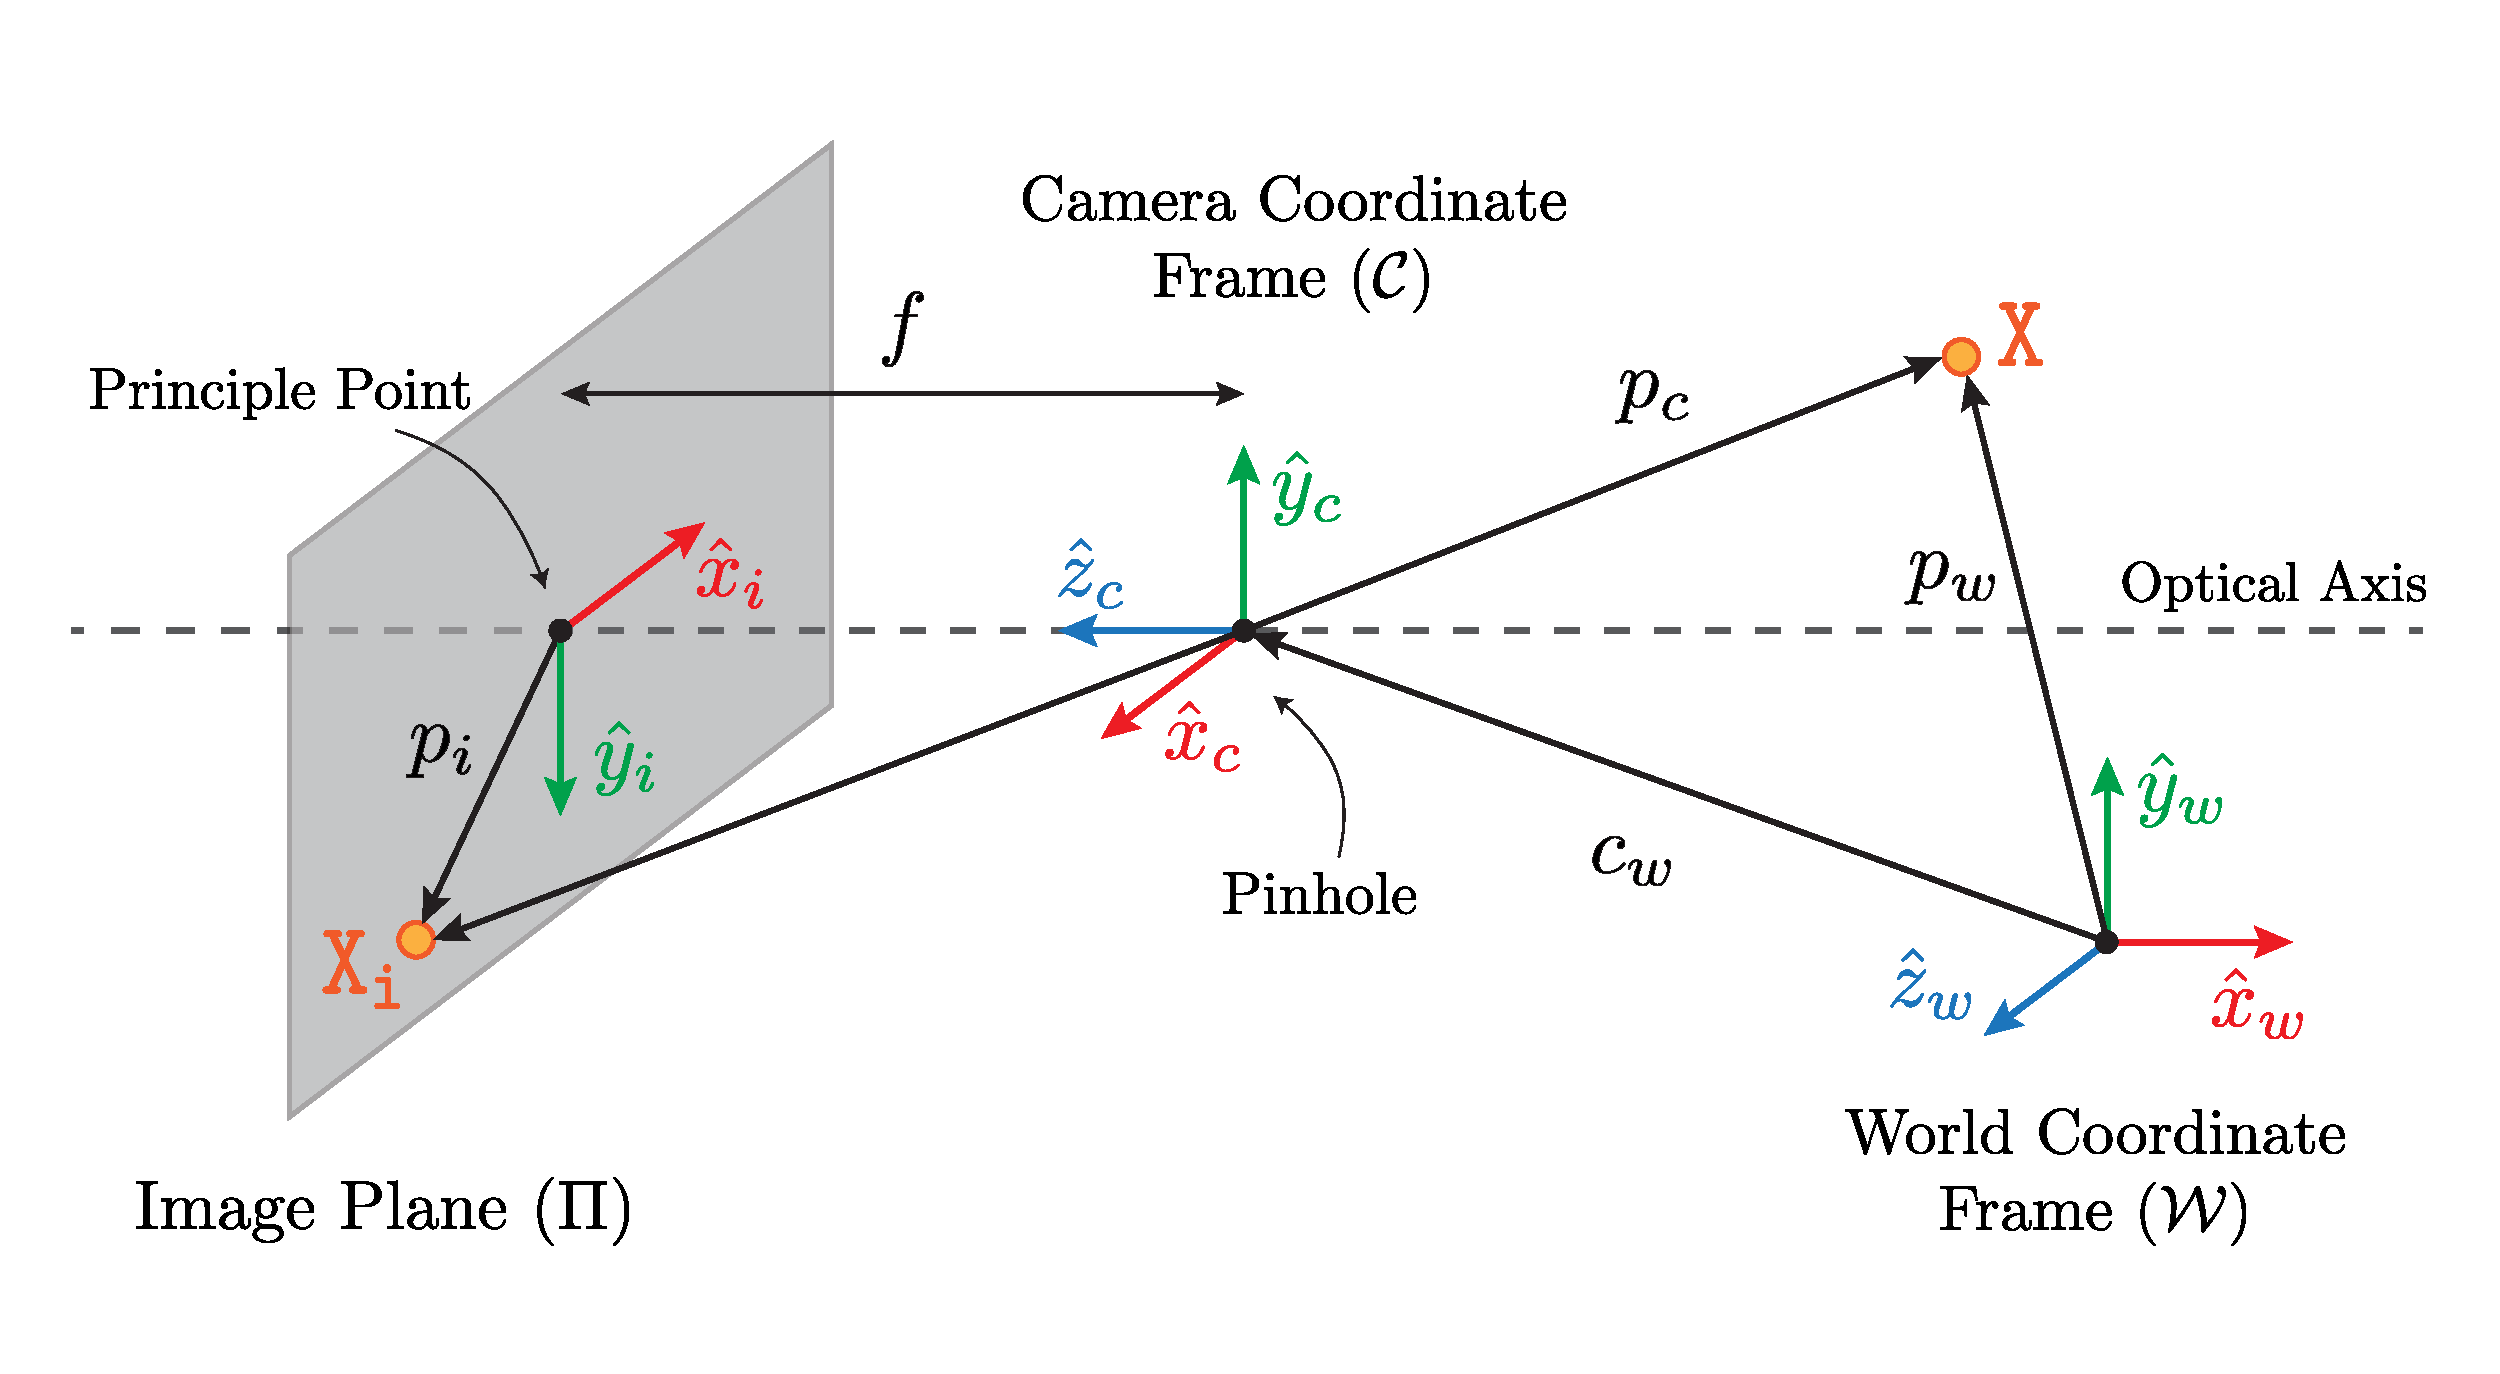
\includegraphics[width=0.9\textwidth]{figures/imaging_model}
    \caption{Pinhole camera model.}
\end{figure}



\begin{figure}[h!]
    \centering
    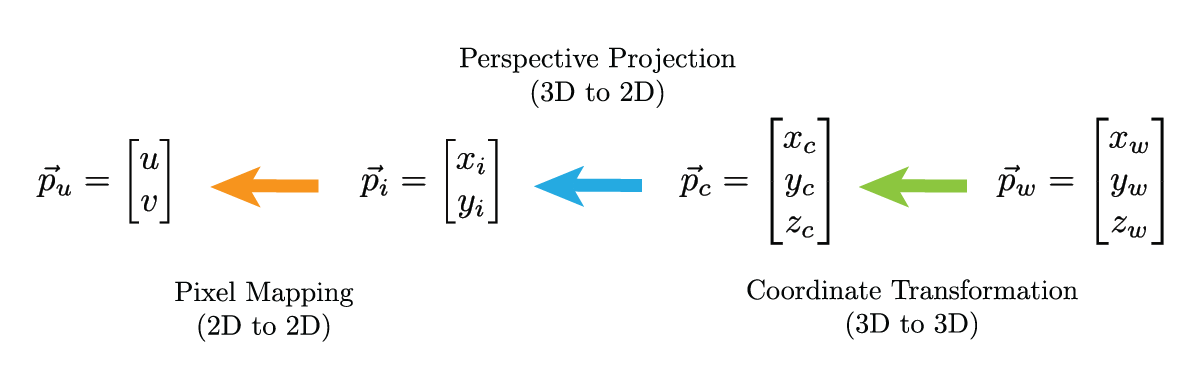
\includegraphics[width=0.9\textwidth]{figures/coord_conversions}
    \caption{Coordinate remappings.}
\end{figure}



